\chapter {Felhasználói dokumentáció}
\label{ch:user}

A felhasználói dokumentáció során először írni fogok a kipróbálóprogram használatáról, melyben röviden bemutatom a funkcionalitását és hogy hogyan működik. Ez után mivel a komponens felhasználói is programozók, látható lesz egy rövid összefoglaló a publikus API\footnote{Application Programming Interface} -ról és annak helyes használatáról. Ezt szükségesnek érzem mivel egy jó API elkészítése külön kihívást jelentő feladat. Akkor jó egy API, ha azt lehetetlen rosszul használni, tartja a mondás. Ez sajnos az életben nem mindig kivitelezhető, ezért érdemes az API-jainkhoz megfelelő dokumentációt készíteni.

\section{Teszt program}

A tesztprogram működése a lehető legegyszerűbben hivatott szemléltetni az alkalmazás funkcionalitását, ebből kifolyólag a minimalista dizájn mellett döntöttem és egy számomra nagyon emlékezetes adatbázis sémán dolgozok in memory\footnote{Teljes adatbázis leképezés memóriában} módon, ez pedig nem más, mint az Adatbázisok 1 során megismert szeret tábla. A tábla tartalmaz Micimackó szereplőket és gyümölcsöket, a köztük lévő reláció pedig jelképezi, hogy a mesefigura szereti-e az adott gyümölcsöt. Ez az egyszerűsége miatt reményem szerint mindenki számára érthető módon szemlélteti majd a háttérben lezajló komplex folyamatokat.

A tesztprogram felhasználói interfésze a következőképpen épül fel:
\begin{itemize}
	\item Fő ablak
    \begin{itemize}
    	\item Felhasználók tab
    	\item Gyümölcsök tab
    \end{itemize}
	\item Felhasználó – Gyümölcs reláció kezelő dialógus
\end{itemize}

A következő részben az egyes komponensek részletezése következik.

\subsection{Hordozható alkalmazás}

Az alkalmazás portable módon próbálható ki, ami azt jelenti, hogy a futtatható állományt nem szükséges telepíteni a számítógépekre.

\subsection{Fő ablak}

A fő ablak tartalmazza az összes komponensét az alkalmazásunknak, amellyel interakcióba léphetünk. Felül a menüsávban az Edit relations menü elem segítségével szerkeszthetjük meg a kapcsolatainkat. Ez a dialógus résznél tovább lesz részletezve. Lejjebb az alkalmazás 2 fő tabból épül fel, amik között válthatunk megszorítások nélkül balegérgombbal történő kattintás segítségével.

\begin{figure}[H]
	\centering
	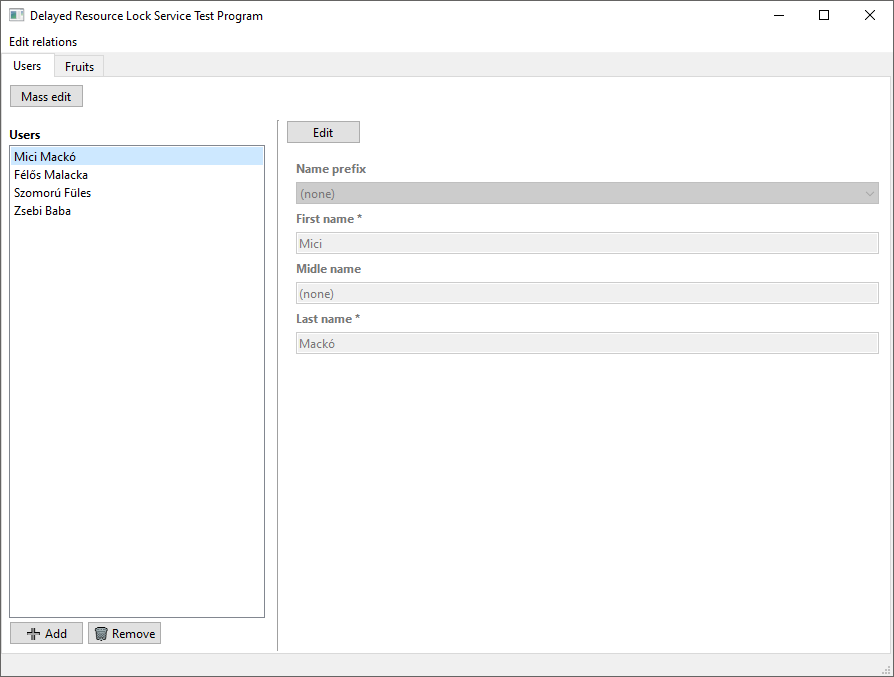
\includegraphics[width=1\textwidth]{images/UsersTab.png}
	\caption{Fő ablak}
	\label{fig:main_window}
\end{figure}

\subsection{Felhasználók tab}

A felhasználók tab egy úgynevezett master detail nézetű szerkesztő felületet valósít meg a felhasználók felett. A tab bal oldalán található egy listás megjelenítés, amiben a felhasználók nevei olvashatóak. A lista alatt található Add gombbal adhatunk hozzá új felhasználót a rendszerhez ez alapértelmezetten "New User" néven jön létre. Ugyancsak a lista alatt látható egy Remove feliratú gomb is, aminek a megnyomása a kiválasztott listaelem és azzal együtt a felhasználó törlését eredményezi.

A táblázatban lévő elemek kiválasztásával a details részen látható űrlap komponensei kitöltődnek a felhasználóra jellemző tulajdonságokkal, ez esetünkben a Név előtagja (Name prefix), Keresztnév (First name), Középső név (Middle name) és Vezetéknév (Last name) mezők. Ezek a komponensek alapból letiltott módban vannak, kijelölésük, szerkesztésük nem lehetséges.

\begin{figure}[H]
	\centering
	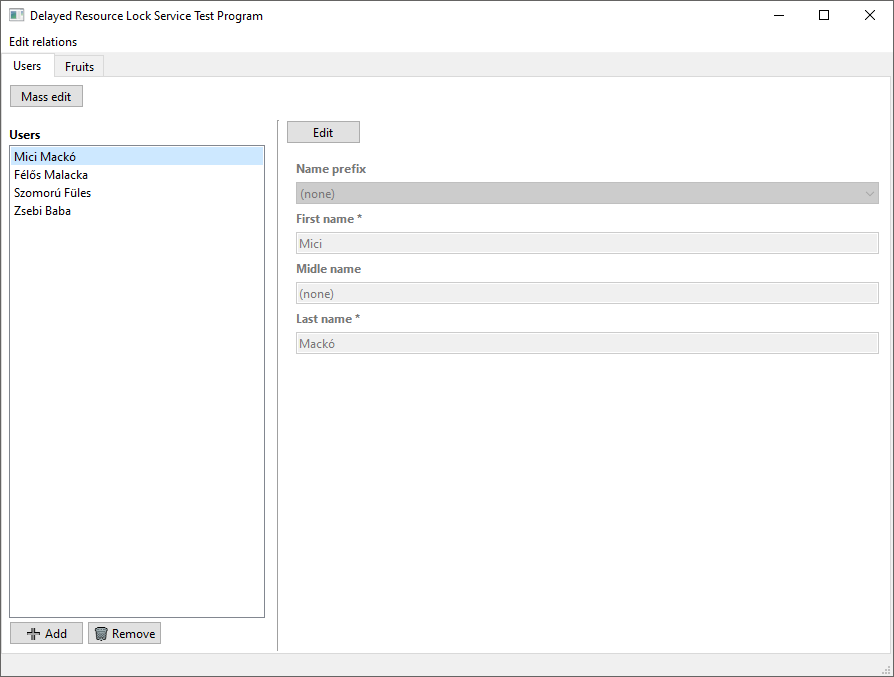
\includegraphics[width=1\textwidth]{images/UsersTab.png}
	\caption{Felhasználók tab}
	\label{fig:main_window}
\end{figure}

A szerkesztésre is van természetesen lehetőség, kettő féleképpen is. Az egyik mód a közvetlenül a mezők felett elhelyezett Edit gomb megnyomásával lehetséges. Ez az alkalmazásunkat az úgynevezett Single Edit módba helyezi. Ebben az állapotban lehetőségünk van az általunk kiválasztott elemet szerkeszteni, de csak azt. Az Edit gomb helyett megjelennek az ehhez a módhoz tartozó specifikus gombok a Save és a Revert. A szerkesztés végeztével ezek segítségével menthetjük el vagy állíthatjuk vissza a szerkesztett felhasználót korábbi állapotába, ha nem szeretnénk megtartani a változtatásokat.

\begin{figure}[H]
	\centering
	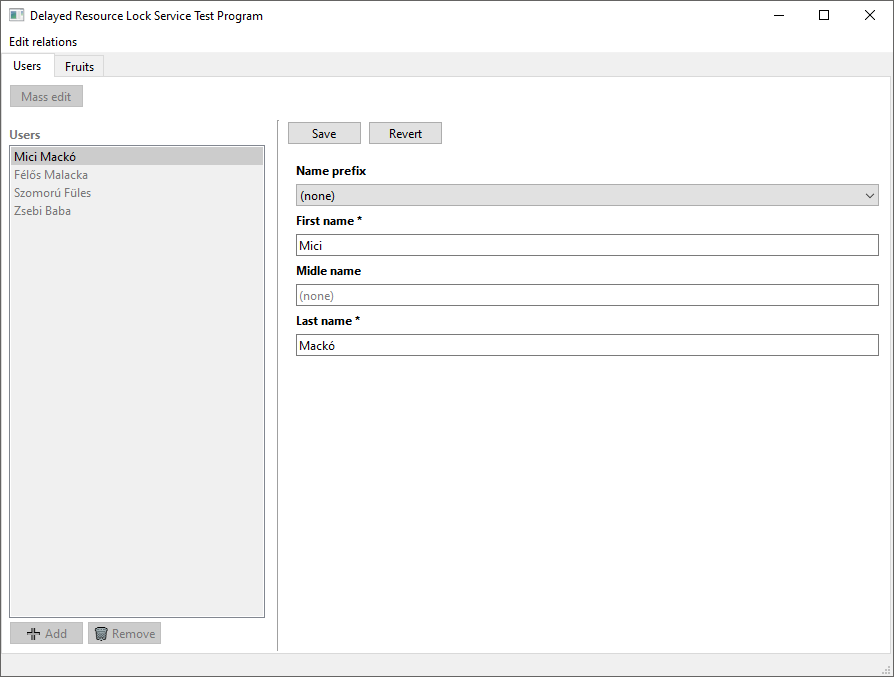
\includegraphics[width=1\textwidth]{images/UsersTabEdit.png}
	\caption{Felhasználók tab szerkesztés alatt}
	\label{fig:main_window}
\end{figure}

A másik lehetőség a tab bal felső sarkába elhelyezett Mass edit gomb megnyomásával érhető el. Ennek segítségével az alkalmazásunk a tömeges szerkesztés állapotba kerül. Ebben az állapotban váltogathatunk a felhasználók között, változtathatunk az attribútumokon, hozzáadhatunk és törölhetünk felhasználót. Az előbb említett felhasználói felületen végzett módosulások azonnal fejtik ki hatásukat, nem szükséges a szerkesztési módból kilépnünk. A tömeges szerkesztés befejezéséhez a bal felső Mass edit gomb helyén megjelenő Finish editing gombbal léphetünk ki. A tömeges szerkesztés módban a beviteli mezők felett közvetlenül elhelyezkedő Edit gomb nem jelenik meg, helyette tájékoztató szöveg olvasható arról, hogy miért nem látható a gomb, ennek az oka természetesen az, hogy egy másik szerkesztési mód jelenleg is aktív.

\begin{figure}[H]
	\centering
	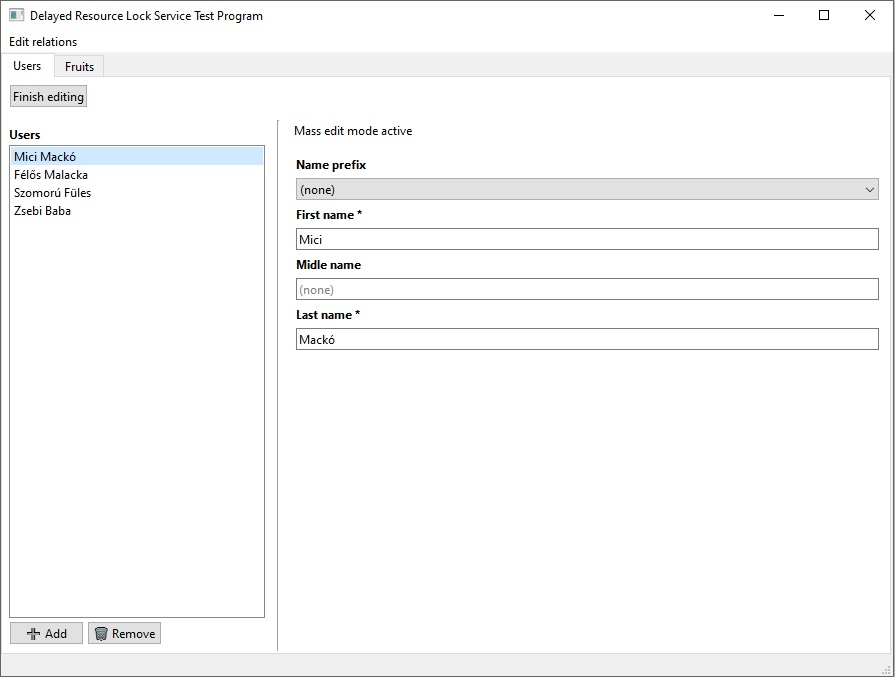
\includegraphics[width=1\textwidth]{images/UsersTabMassEdit.png}
	\caption{Felhasználók tab szerkesztés alatt}
	\label{fig:main_window}
\end{figure}

\subsection{Gyümölcsök tab}

A gyümölcsök tab a felhasználók mintájára készült el, így a működések teljes mértékben megegyeznek a korábbiakban leírtakkal. Az egyetlen főbb különbség, hogy itt a gyümölcsöknek csupán név tulajdonságuk van így annak a változtatásai érvényesülnek a korábbi 4 megemlített helyett.

\subsection{Felhasználó - Gyümölcs relációk szerkesztése}

A főoldal bal felső sarkában található Edit relations lenyíló menüben található egyetlen elem a Fruit - User elem.

\begin{figure}[H]
	\centering
	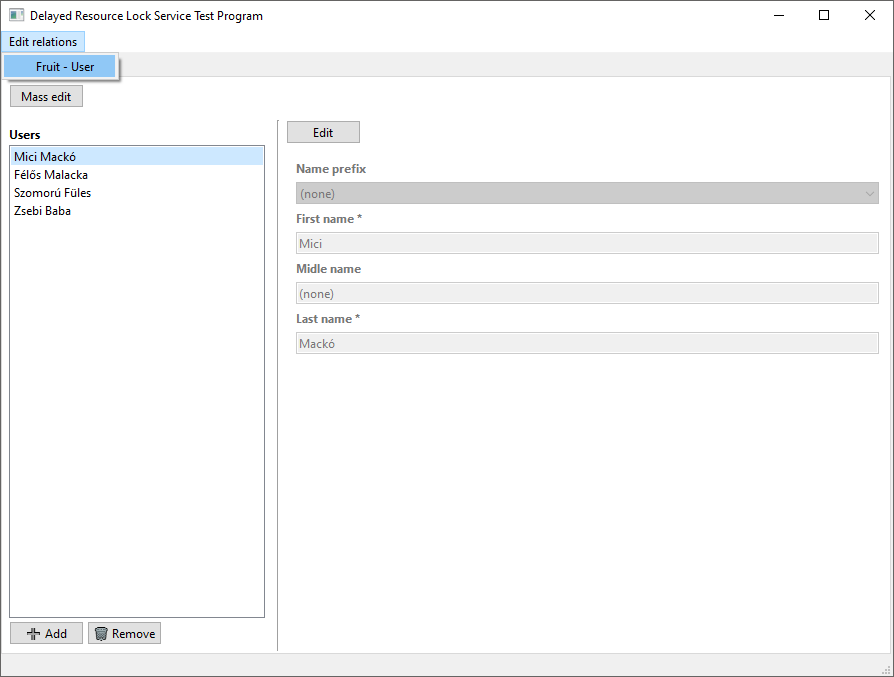
\includegraphics[width=1\textwidth]{images/EditUser-Fruit.png}
	\caption{Fruit - User menü elem}
	\label{fig:main_window}
\end{figure}

Ennek megnyomásával lehetőségünk nyílik a gyümölcsök és felhasználók közti relációk szerkesztésére, amit egy dialóguson keresztül tehetünk meg ebben a dialógusban kettő lista található az oldal bal és jobb oldalán. Az egyik a felhasználóinkat tartalmazza nevük alapján beazonosítható módon, míg a másik hasonlóképpen név szerint a gyümölcsöket tartalmazza. A két listából történő egy-egy elem kiválasztása után a két lista között elérhetővé válik a link vagy az unlink opció annak függvényében, hogy a két általunk választott elem, amelyből az egyik a felhasználó, a másik pedig természetesen a gyümölcs. Ez a gomb állapotában leköveti a kiválasztott elemeink státuszát. Amennyiben az elemek között létezik reláció, ami azt reprezentálja, hogy a 
felhasználó szereti a gyümölcsöt a gomb szövege Unlinkre vált, ami jelöli, hogy a lenyomásával ez a kapcsolat meg fog szűnni. Ennek mintájára, ha a két elem között nem létezik kapcsolat a gomb szövege Link-re vált, amelynek lenyomása kialakítja az elemek közti relációt, szellemesen mondhatjuk, hogy a felhasználóval megszeretteti a gyümölcsöt. A szeretetet reprezentáló reláció meglétére vagy meg nem létére egy másik komponens is felhívja a figyelmünket, ez pedig egy egyszerű szöveges jelölés, ami, a két elem közé egy összeköttetést rak, ha azok relációban állnak egymással, ha viszont nem akkor ezt az összeköttetést a közepénél egy látványos szakadással látjuk megjelenni.

\begin{figure}[H]
	\centering
	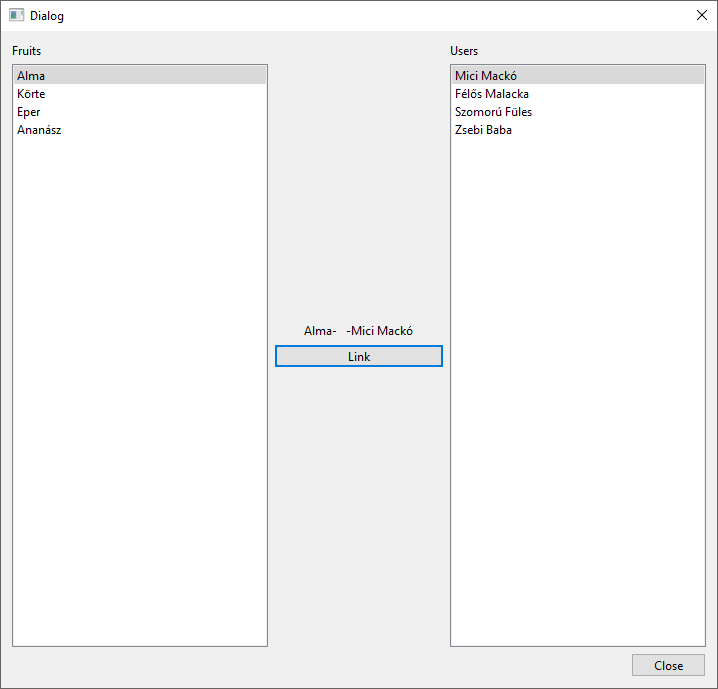
\includegraphics[width=1\textwidth]{images/Link.png}
	\caption{Reláció szerkesztése - Összekapcsolás}
	\label{fig:main_window}
\end{figure}

\begin{figure}[H]
	\centering
	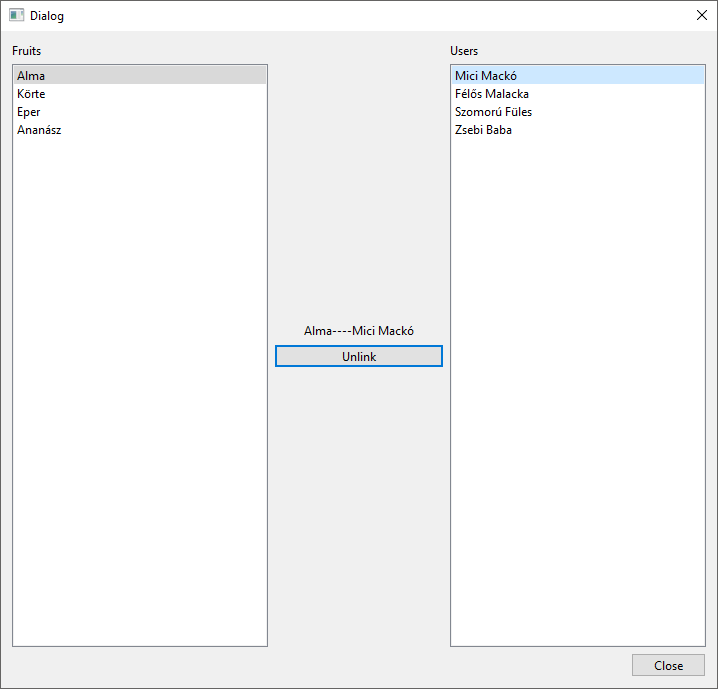
\includegraphics[width=1\textwidth]{images/Unlink.png}
	\caption{Reláció szerkesztése - Szétkapcsolás}
	\label{fig:main_window}
\end{figure}

\section{Egymást kizáró műveletek}

A korábbi szekcióban már említés szinten volt szó a szerkesztés módjairól. Ezeknek az elsőre talán feleslegesnek tűnő műveleteknek az indoklása fog a lentebbi részben következni. A háttérben lévő entitások integritása elengedhetetlen az alkalmazás helyes működésének szempontjából. Kimondottan súlyos programozói hiba lenne, ha az entitások különböző helyekről esetleg különböző logikai szálakból szerkeszthetőek lennének. A program működése kiszámíthatatlanná válna, Inkonzisztencia lépne fel, más helyekről mást látnánk ugyan arról az entitásról. Ennek megelőzése érdekében tekintsünk az entitásainkra úgy, mint erőforrásokra. Az erőforrásainkat kettő féleképpen lehet lefoglalni, írási vagy olvasási preferenciával. A konkurens olvasás megengedett, az írás nem megengedett. Az alkalmazásban explicit módja az entitások erőforrás jellegű lefoglalásának az edit gombok használata. Szerkesztés közben fenntartjuk a zárat, más helyről az azonos entitások nem szerkeszthetőek.

Emellett az alkalmazásban lévő relációk szerkesztése dialógus is, viszont ez implicit módon teszi, zárakat hoz létre az általa szerkesztett entitásokra.

A kipróbáló programunkban lehetőségünk is van ezek megtapasztalására abban az esetben, ha szerkesztés módban nyitjuk meg a relációk szerkesztése dialógusunkat. Ekkor az edit mód által lefoglalt entitásainkat olvasási preferenciájú zárát próbálja meg újra lefoglalni a dialógus, ami nem fog sikerülni mivel ezek nem jöhetnek létre konkurens módon. Az alkalmazásunk ennek sikertelenségéről egy hibaüzenet formájában tájékoztat, amiben leírja, hogy az erőforrások már más birtokában vannak.

\begin{figure}[H]
	\centering
	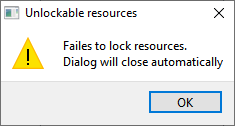
\includegraphics[width=0.4\textwidth]{images/Unlockable.png}
	\caption{Zárolási hibaüzenet dialógus megnyitása esetén}
	\label{fig:main_window}
\end{figure}